\section{Đánh giá DataWarehouse}
\subsection{Đánh giá mức độ tiêu thụ tài nguyên của luồng nạp dữ liệu khối lượng lớn}

Nhằm đánh giá khả năng xử lý của hệ quản trị cơ sở dữ liệu trên nền tảng Azure Database for PostgreSQL, nhóm tiến hành thực nghiệm với kịch bản nạp dữ liệu quy mô lớn (\textit{Bulk Ingestion}), tương đương khoảng 3 GB dữ liệu, tương ứng xấp xỉ 30 triệu bản ghi. Quá trình thực nghiệm được theo dõi thông qua hệ thống giám sát Azure Monitor nhằm ghi nhận mức độ sử dụng tài nguyên và trạng thái hoạt động của cơ sở dữ liệu.

Kết quả quan sát cho thấy mức sử dụng CPU cực đại đạt khoảng $86.5\%$, trong khi mức sử dụng bộ nhớ duy trì ổn định quanh ngưỡng $66\%$. Dung lượng lưu trữ còn trống ở mức an toàn và không ghi nhận hiện tượng vượt ngưỡng bộ nhớ hay sự cố dừng dịch vụ. Trong suốt quá trình thực nghiệm, cơ sở dữ liệu duy trì trạng thái sẵn sàng hoạt động, không xuất hiện kết nối thất bại và toàn bộ dữ liệu đều được ghi nhận thành công.

Kết quả này cho thấy cấu hình hiện tại của hệ thống có khả năng đáp ứng các tác vụ nạp dữ liệu quy mô lớn, đồng thời vẫn duy trì được tính ổn định trong trường hợp cần thực hiện quá trình đồng bộ lại dữ liệu (\textit{Backfill}) sau các khoảng thời gian gián đoạn kết nối kéo dài.

\begin{figure}[H]
    \centering
    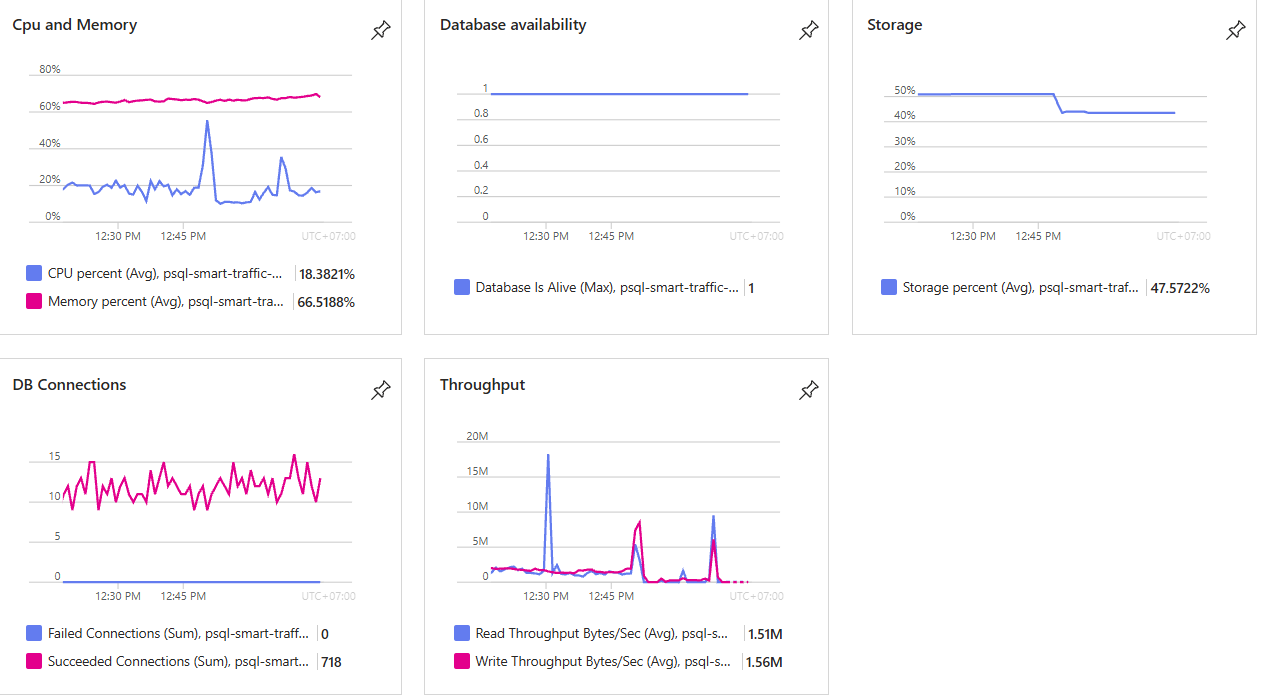
\includegraphics[width=\linewidth]{Images/azuretongquan.png}
    \caption{Các chỉ số giám sát tổng quan của Azure Database for PostgreSQL trong quá trình thực hiện Bulk Ingestion}
    \label{fig:azure_monitor_overview}
\end{figure}

\subsection{Đánh giá khả năng chịu tải của hạ tầng lưu trữ và tài nguyên tính toán}

Để khảo sát ảnh hưởng của tải ghi dữ liệu lớn lên hạ tầng Data Warehouse, nhóm tiến hành thực nghiệm \textit{Stress Test} bằng cách tạo ra luồng Ingestion liên tục với cường độ cao. Các chỉ số về mức sử dụng CPU và hoạt động nhập/xuất được thu thập từ Azure Monitor nhằm xác định các thành phần có khả năng trở thành nút thắt hiệu năng.

Kết quả cho thấy mức sử dụng CPU xuất hiện nhiều giai đoạn tăng cao, với giá trị cực đại khoảng $86.5\%$. Điều này phản ánh khối lượng tính toán đáng kể mà hệ quản trị cơ sở dữ liệu phải thực hiện trong quá trình xử lý dữ liệu, bao gồm các thao tác chuyển đổi dữ liệu, gán nhãn thời gian và xử lý các thuộc tính không gian thông qua phần mở rộng PostGIS. Tuy nhiên, hệ thống chưa xuất hiện trạng thái bão hòa tài nguyên xử lý.

\begin{figure}[H]
    \centering
    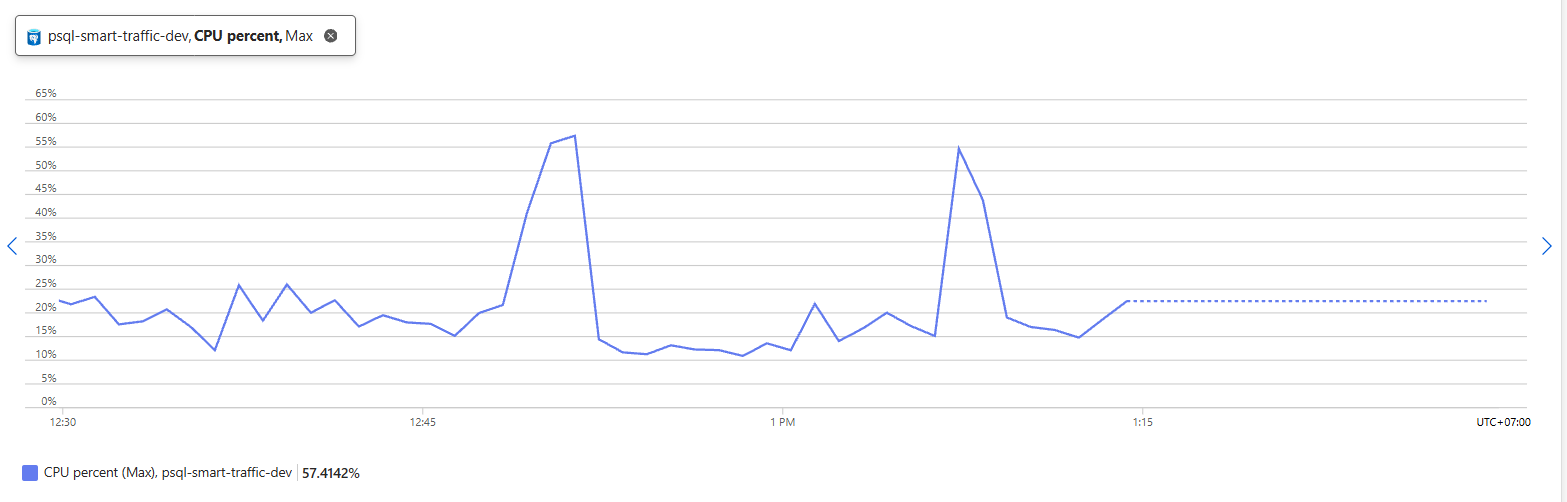
\includegraphics[width=\linewidth]{Images/CPUmax.png}
    \caption{Mức sử dụng CPU cực đại của Azure Database for PostgreSQL trong quá trình nạp dữ liệu khối lượng lớn}
    \label{fig:cpu_bulk_ingestion}
\end{figure}

Đối với tầng lưu trữ, chỉ số IOPS dao động quanh khoảng $750$--$800$ thao tác mỗi giây và đạt giá trị cực đại xấp xỉ $1000$ IOPS trong thời gian thực nghiệm. Kết quả này cho thấy áp lực ghi dữ liệu lên hệ thống lưu trữ tăng đáng kể khi khối lượng dữ liệu đầu vào lớn. Tuy nhiên, chưa ghi nhận dấu hiệu suy giảm hiệu năng hoặc hiện tượng nghẽn tài nguyên lưu trữ rõ rệt trong phạm vi thử nghiệm.

\begin{figure}[H]
    \centering
    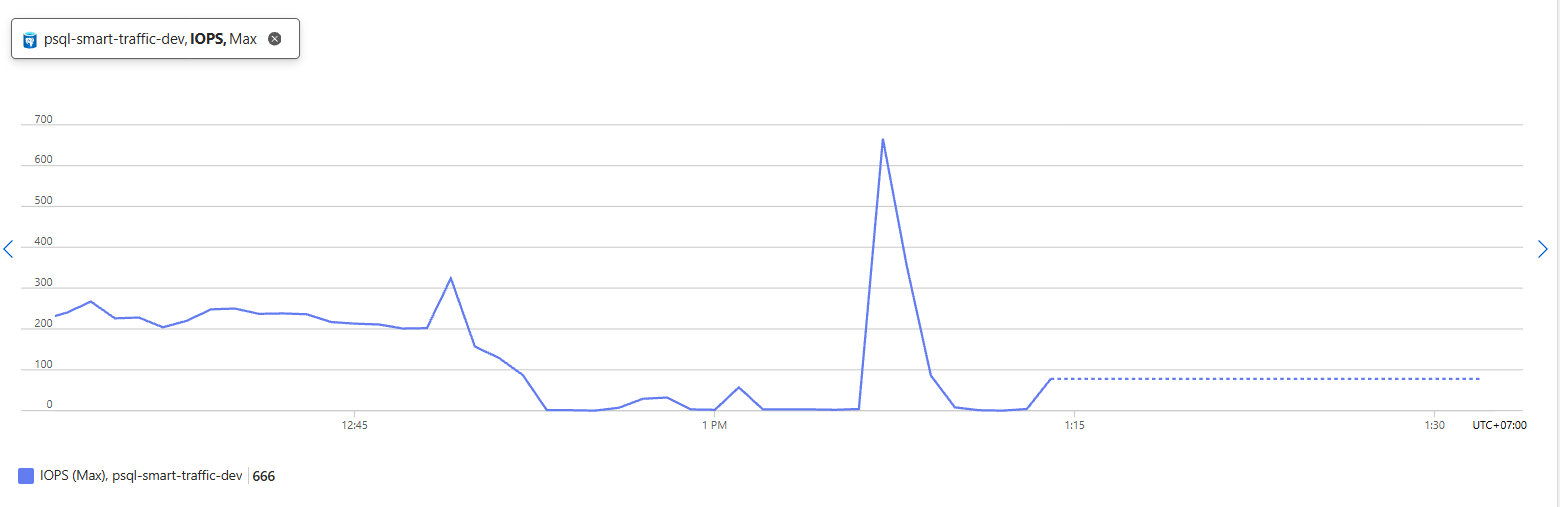
\includegraphics[width=\linewidth]{Images/IOPSmax.png}
    \caption{Biến thiên chỉ số IOPS trong quá trình thực hiện Stress Test}
    \label{fig:iops_bulk_ingestion}
\end{figure}

Nhìn chung, kết quả thực nghiệm cho thấy kiến trúc hiện tại đáp ứng tốt tải vận hành thông thường cũng như các tác vụ đồng bộ dữ liệu quy mô lớn. Tuy nhiên, khi khối lượng dữ liệu tiếp tục gia tăng trong tương lai, việc tối ưu cơ chế nạp dữ liệu theo lô (\textit{Batch Processing}), phân vùng dữ liệu và mở rộng tài nguyên tính toán hoặc lưu trữ sẽ là những hướng cải tiến cần được xem xét nhằm duy trì hiệu năng của hệ thống.

\subsection{Đánh giá khả năng đáp ứng đối với tải truy vấn phân tích}

Bên cạnh tải ghi dữ liệu, nhóm tiến hành đánh giá khả năng phản hồi của hệ thống trước các truy vấn phân tích thường gặp trong các ứng dụng trực quan hóa dữ liệu và hệ thống báo cáo. Kịch bản thực nghiệm được xây dựng với nhiều người dùng truy cập đồng thời, thực hiện các truy vấn tổng hợp sử dụng các phép toán \texttt{GROUP BY}, \texttt{AVG} và \texttt{MAX} trên tập dữ liệu gồm khoảng 432\,000 bản ghi.

Kết quả thực nghiệm cho thấy thời gian phản hồi của các truy vấn dao động từ khoảng $0.7$ giây đến $2.8$ giây. Sự khác biệt này chủ yếu xuất phát từ trạng thái của cơ chế bộ nhớ đệm (\textit{Shared Buffers}) và mức độ sử dụng tài nguyên của hệ thống tại từng thời điểm. Đồng thời, các chỉ số giám sát cho thấy tải xử lý của CPU tăng lên đáng kể trong quá trình thực hiện các phép tổng hợp trên dữ liệu.

\begin{table}[H]
\centering
\caption{Thời gian phản hồi của các truy vấn phân tích}
\label{tab:query_time}
\begin{tabular}{|c|c|}
\hline
Lần thực thi & Thời gian phản hồi (s) \\
\hline
1 & 2.794 \\
2 & 1.098 \\
3 & 0.772 \\
\hline
\end{tabular}
\end{table}

Mặc dù thời gian phản hồi vẫn nằm trong phạm vi chấp nhận được đối với các tác vụ phân tích, kết quả thực nghiệm cho thấy chi phí tính toán có xu hướng gia tăng khi kích thước dữ liệu tăng lên. Do đó, việc thực hiện các truy vấn tổng hợp trực tiếp trên các bảng Fact với quy mô lớn có thể làm gia tăng độ trễ và ảnh hưởng đến khả năng mở rộng của hệ thống trong tương lai.

Từ kết quả này, nhóm lựa chọn kiến trúc xử lý đa tầng nhằm giảm tải cho cơ sở dữ liệu. Cụ thể, các chỉ số tổng hợp thường xuyên được truy cập được tính toán trước thông qua \textit{Materialized View} kết hợp với các cấu trúc chỉ mục phù hợp. Bên cạnh đó, một lớp bộ nhớ đệm tại tầng ứng dụng, chẳng hạn như Redis hoặc MongoDB Cache, có thể được tích hợp nhằm giảm số lượng truy vấn trực tiếp đến Data Warehouse, từ đó cải thiện khả năng đáp ứng của hệ thống đối với người dùng cuối.

\begin{table}[H]
\centering
\caption{Tóm tắt kết quả đánh giá hiệu năng của hệ thống}
\label{tab:performance_summary}
\begin{tabular}{|p{5cm}|c|}
\hline
Chỉ số & Giá trị quan sát được \\
\hline
Dung lượng dữ liệu thử nghiệm & $\sim$3 GB ($\sim$30 triệu bản ghi) \\
\hline
CPU cực đại & 86.5\% \\
\hline
Mức sử dụng bộ nhớ trung bình & 66\% \\
\hline
IOPS cực đại & 997 \\
\hline
Read Throughput trung bình & 1.51 MB/s \\
\hline
Write Throughput trung bình & 1.56 MB/s \\
\hline
Failed Connections & 0 \\
\hline
Database Availability & 100\% \\
\hline
Thời gian phản hồi truy vấn & 0.772 -- 2.794 s \\
\hline
\end{tabular}
\end{table}

\subsection{Nhận xét tổng quát}

Thông qua các kịch bản kiểm thử tải ghi dữ liệu và tải truy vấn phân tích, kết quả thực nghiệm cho thấy hệ thống Data Warehouse được xây dựng trên Azure Database for PostgreSQL có khả năng vận hành ổn định trong điều kiện tải thực tế của bài toán. Các chỉ số về CPU, bộ nhớ, lưu trữ và khả năng phản hồi đều nằm trong giới hạn chấp nhận được và chưa xuất hiện dấu hiệu mất ổn định hay suy giảm hiệu năng nghiêm trọng.

Tuy nhiên, khi quy mô dữ liệu tiếp tục tăng lên theo thời gian, việc áp dụng các kỹ thuật tối ưu như tiền tính toán (\textit{pre-aggregation}), \textit{Materialized View}, cơ chế bộ nhớ đệm, phân vùng dữ liệu và mở rộng tài nguyên hạ tầng sẽ đóng vai trò quan trọng trong việc đảm bảo tính mở rộng và duy trì hiệu năng của hệ thống trong dài hạn.
